\documentclass[preprint]{acm_proc_article-sp}
%\documentclass[preprint]{sig-alternate}
\usepackage{url}
\usepackage{graphicx,subfigure}
\usepackage{xspace}

\newcommand{\ie}{{\em i.e.,}~}
\newcommand{\eg}{{\em e.g.,}~}
\newcommand{\HadoopBM}{HadoopBinMem\xspace}

\newenvironment{denseitemize}{
\begin{itemize}[topsep=2pt, partopsep=0pt, leftmargin=1.5em]
  \setlength{\itemsep}{4pt}
  \setlength{\parskip}{0pt}
  \setlength{\parsep}{0pt}
}{\end{itemize}}

\begin{document}

\title{Shark: Fast Data Analysis Using Coarse-grained Distributed Memory}

\numberofauthors{5}
\author{
Cliff Engle,
Antonio Lupher,
Reynold Xin,
Matei Zaharia,\\
Michael Franklin,
Scott Shenker,
Ion Stoica\\\\
AMPLab, EECS, UC Berkeley\\
\texttt{\{cengle, alupher, rxin, matei, franklin, shenker, istoica\}@cs.berkeley.edu}
}

\maketitle
\begin{abstract}
Shark is a research data analysis system built on a novel coarse-grained distributed shared-memory abstraction. Shark marries query processing with deep data analysis, providing a unified system for easy data manipulation using SQL and pushing sophisticated analysis closer to data. It scales to thousands of nodes in a fault-tolerant manner. Shark can answer queries 40X faster than Apache Hive and run machine learning programs 25X faster than MapReduce programs in Apache Hadoop on large datasets.
\end{abstract}

% A category with the (minimum) three required fields
\category{H.2}{Database Management}{Systems}

\terms{DESIGN, MANAGEMENT}

\keywords{Databases, Data Warehouse, Machine Learning}


%%%%%%%%%%%%%%%%%%%%%%%%%%%%%%%%%%%%%%%%%%%%%%%%%%%%%%%%%%%%%%%%%%%%%%%%%%%%%%%
%%%%%%%%%%%%%%%%%%%%%%%%%%%%%%%%%%%%%%%%%%%%%%%%%%%%%%%%%%%%%%%%%%%%%%%%%%%%%%%
%%%%%%%%%%%%%%%%%%%%%%%%%%%%%%%%%%%%%%%%%%%%%%%%%%%%%%%%%%%%%%%%%%%%%%%%%%%%%%%

\section{Introduction}

Modern data analysis employs statistical methods that go well beyond the roll-up and drill-down capabilities provided by traditional enterprise data warehouse (EDW) solutions. Data scientists appreciate the ability to use SQL for simple data manipulation but rely on other systems for machine learning on these data. What is needed is a system that consolidates both. For sophisticated data analysis at scale, it is important to exploit in-memory computation.  This is particularly true with machine learning algorithms that are iterative in nature and exhibit strong temporal locality. Main-memory database systems use a \emph{fine-grained} memory abstraction in which records can be updated individually. This fine-grained approach is difficult to scale for massive datasets to hundreds or thousands of nodes in a fault-tolerant manner. In contrast, a \emph{coarse-grained abstraction}, in which transformations are performed on an entire collection of data, has been shown to scale more easily
\footnote{MapReduce is an example of coarse-grained updates as the same map and reduce functions are executed on all records.}.

\subsection{Coarse-grained Distributed Memory}
We have previously proposed a new distributed memory abstraction for in-memory computations on large clusters called Resilient Distributed Datasets (RDDs) \cite{spark-tr}. RDDs provide a restricted form of shared memory, based on coarse-grained transformations on immutable collections of records rather than fine-grained updates to shared states. RDDs can be made fault-tolerant based on lineage information rather than replication. When the workload exhibits temporal locality, programs written using RDDs outperform systems such as MapReduce by orders of magnitude. Surprisingly, although restrictive, RDDs have been shown to be expressive enough to capture a wide class of computations, ranging from more general models like MapReduce to more specialized models such as Pregel.

It might seem counterintuitive to expect memory-based solutions to help when petabyte-scale data warehouses prevail. However, it is unlikely, for example, that an entire EDW fact table is needed to answer most queries. Queries usually focus on a particular subset or time window, \eg http logs from last month, touching only the (small) dimension tables and a small portion of the fact table. Thus, in many cases it is plausible to fit the working set into a cluster's memory. In fact, \cite{memento-hotos} analyzed the access patterns in the Hive warehouses at Facebook and discovered that for the vast majority (96\%) of jobs, the entire inputs could fit into a fraction of the cluster's total memory.

\subsection{Introducing Shark}
The goal of the Shark (Hive on Spark) project is to design a data warehouse system capable of deep data analysis using the RDD memory abstraction. It unifies the SQL query processing engine with analytical algorithms based on this common abstraction, allowing the two to run in the same set of workers and share intermediate data.

Apart from the ability to run deep analysis, Shark is much more flexible and scalable compared with EDW solutions. Data need not be extracted, transformed, and loaded into the rigid relational form before analysis. Since RDDs are designed to scale horizontally, it is easy to add or remove nodes to accommodate more data or faster query processing. The system scales out to thousands of nodes in a fault-tolerant manner. It can recover from node failures gracefully without terminating running queries and machine learning functions.

Compared with disk-oriented warehouse solutions and batch infrastructures such as Apache Hive \cite{hive}, Shark excels at ad-hoc, exploratory queries by exploiting inter-query temporal locality and also leverages the intra-query locality inherent in iterative machine learning algorithms. By efficiently exploiting a cluster's memory using RDDs, queries previously taking minutes or hours to run can now return in seconds. This significant reduction in time is achieved by caching the working set of data in a cluster's memory, eliminating the need to repeatedly read from and write to disk.

In the remainder of this demonstration proposal, we sketch Shark's system design and give a brief overview of the system's performance. Finally, we describe in detail how we plan to demonstrate Shark at SIGMOD. Due to space constraints, we refer readers to \cite{spark-tr} for more details on RDDs.

%\subsection{RDDs}
%RDDs provide a restricted form of shared memory, based on coarse-grained transformations on immutable collections of records rather than fine-grained updates to shared states. When the workload exhibits temporal locality, programs written using RDDs outperform by orders of magnitude programs written for other system such as MapReduce. And surprisingly, although restrictive, RDDs have been shown to be expressive enough to capture a wide class of computations, ranging from more general models like MapReduce to more specialized models such as Pregel.

%Formally, an RDD is an immutable, partitioned collection of records that can only be created through deterministic \emph{transformations} on either data in stable storage (\eg files in HDFS) or other RDDs. Examples of transformations include \emph{map}, \emph{filter}, \emph{reduce}, and \emph{join}. Note that RDDs do not need to be materialized at all times, as they can be reconstructed based on lineage information. Users can control two aspects of RDDs: \emph{persistence} and \emph{partitioning}. Using the persistence API, users can indicate which RDDs they will reuse and choose a storage strategy for them (\eg caching them in memory). This is particularly useful in cache investment as the higher level program can choose to materialize certain RDDs in memory and reuse them later. For workloads that require going through data multiple times, such as interactive queries and iterative machine learning queries, Spark's persistence feature is very attractive. They can also ask that an RDD's elements be partitioned across machines based on key in each record. This is useful for placement optimizations, such as ensuring that two datasets that will be joined together are hash-partitioned in the same way.



%Data scientists, however, appreciate using SQL to manipulate data. Traditionally, they load data into a relational database for basic analysis, and then run algorithms in external computation frameworks such as MapReduce. Shark allows the users to express deep analyses as well as simple SQL queries, and the two can effectively share the same computation resource as well as the same in-memory data.

%Although Hive was designed to be a data warehousing solution, based on our discussions with many Hive users, a large percentage of Hive queries are ad-hoc, exploratory in nature and issued from the Hive console rather than programmatically generated for traditional data warehousing reports. Take Facebook for example. Their Hadoop clusters are dominated by jobs generated from Hive \cite{hive} queries. Even though the queries are intended to be exploratory, median map and reduce job duration is 84s \cite{delay-scheduling}. Note that typical query duration would be a multiple of this number since a query consists of multiple stages of map and reduce jobs. There is a tremendous difference in interactivity between queries that run in seconds versus minutes or hours.


%%%%%%%%%%%%%%%%%%%%%%%%%%%%%%%%%%%%%%%%%%%%%%%%%%%%%%%%%%%%%%%%%%%%%%%%%%%%%%%
%%%%%%%%%%%%%%%%%%%%%%%%%%%%%%%%%%%%%%%%%%%%%%%%%%%%%%%%%%%%%%%%%%%%%%%%%%%%%%%
%%%%%%%%%%%%%%%%%%%%%%%%%%%%%%%%%%%%%%%%%%%%%%%%%%%%%%%%%%%%%%%%%%%%%%%%%%%%%%%
\section{System Overview}

For ease of adoption, we have designed Shark to be entirely hot-swappable with Hive. Anyone can have Shark up and running in an existing Hive warehouse. Queries will return the same set of results in Shark, albeit much faster, without any modification to data or the queries themselves.

We have implemented Shark using Spark, a system that provides the RDD abstraction through a language-integrated API in Scala (a statically typed functional programming language for the Java VM). Each RDD dataset is represented as a Scala object, while the transformations are invoked using methods on those objects. A Shark cluster consists of masters and workers. A master's lifetime can span one or several queries. The workers are long-lived processes that can store dataset partitions in memory across operations. When the user runs a query, the client connects to a master, which defines RDDs for the workers and invoke operations on them.

Figure \ref{fig:arch} shows the general architecture of Shark. Data are stored physically in the underlying distributed file system HDFS. The Hive metastore is used without modification in Shark and tracks the metadata and statistics about tables, much like the system catalog found in traditional RDBMS. 

\subsection{Query Processing}
From a higher level, Shark's query execution consists of three steps similar to traditional RDBMS: query parsing, logical plan generation, and physical plan generation. Hive provides a SQL-like declarative query language, HiveQL, which gets compiled into lower level operators that are executed in a sequence of MapReduce programs. Shark uses Hive as a third-party Java library for query parsing and logical plan generation. The main difference is in the physical plan execution, as Shark has its own operators written specifically to exploit the benefits provided by RDDs.

\begin{figure}[t]
	\centering
	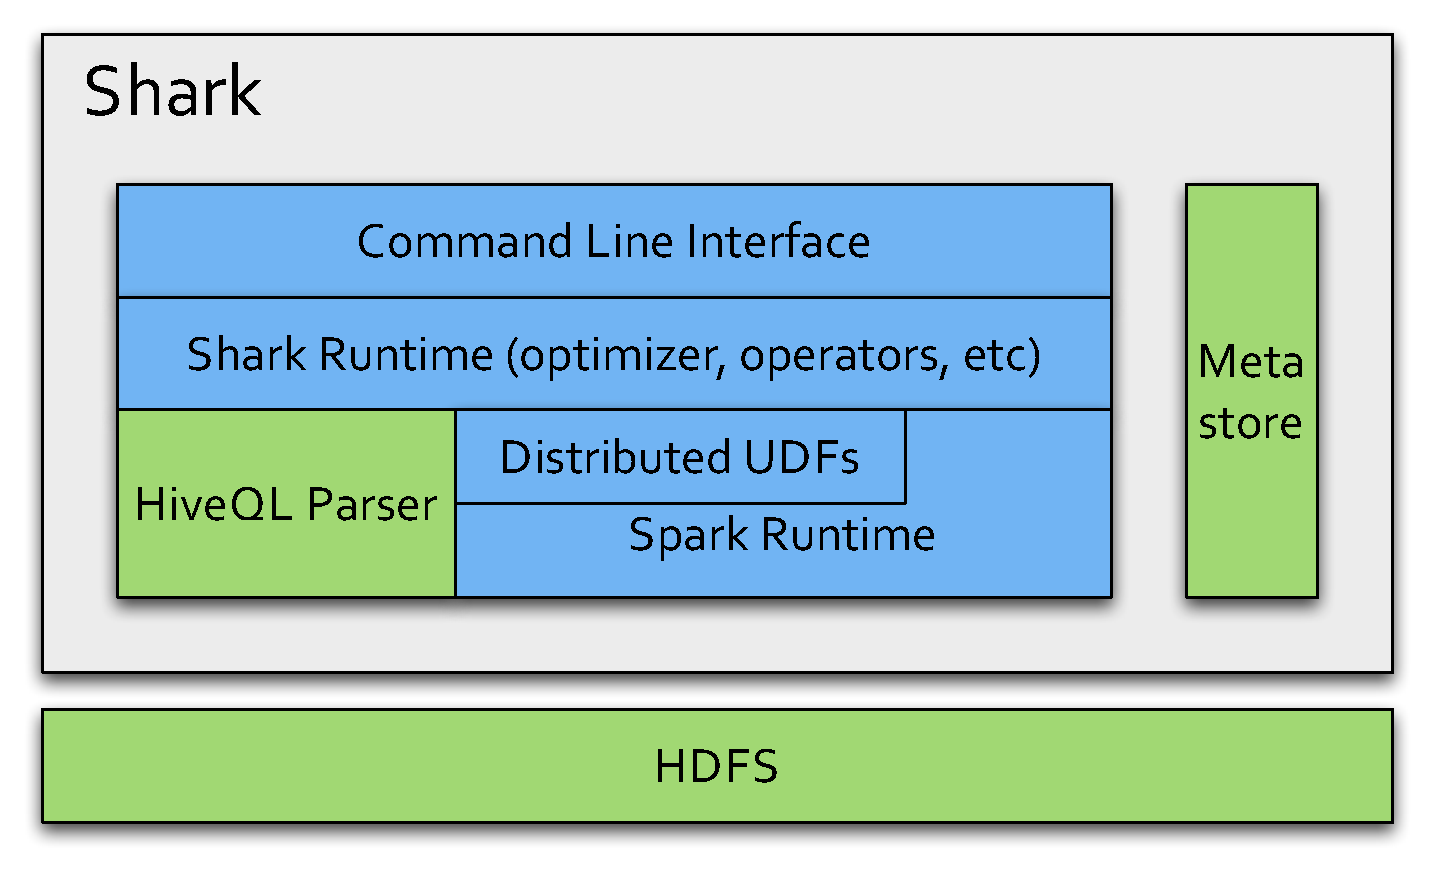
\includegraphics[width=\linewidth]{files/architecture.pdf}
	\caption{Shark Architecture}
	\label{fig:arch}
\end{figure}

Given a HiveQL query, the Hive query compiler is used to parse the query and generate an abstract syntax tree. The tree is then turned into the logical plan and basic logical optimization such as predicate push downs is applied. Up to this point, Shark and Hive follow an identical process. In Hive, this operator tree would be converted into a physical plan that consists of subtrees for separate map reduce tasks. In contrast, in Shark, this operator tree is converted into operators that perform transformations on RDDs. An iterator traverses the operator tree and produces an immutable RDD for each operator on the tree. This RDD is not materialized until the execution engine returns the query results. 

Much of the common structure of Hive operators is retained in order to ensure interoperability with HiveQL. We have currently implemented support for all of the essential Hive operators. We reuse all of Hive's data model and type system, in addition to supporting Hive's user-defined functions, user-defined aggregate functions, custom types, and custom serialization/deserialization methods.

A major advantage of Shark over Hive is the inter-query caching of data. The Spark framework provides a simple mechanism to cache RDDs in memory across clusters and recompute RDDs in the event of failures. In Shark, each operator subtree's result is cached automatically, and a signature is computed for the subtree. This signature, along with a timestamp of the original file's last modification time in HDFS, is stored in a table in the metastore. Signatures are computed for subsequent query subtrees and are compared to those in the table and, in case of a match, the in-memory RDD is utilized. Cache invalidation is handled by checking the timestamp of the last modification of the HDFS data to the timestamp stored in our table. We have implemented a variety of simple cache replacement algorithms such as LFU and LRU, and are currently exploring more sophisticated algorithms that perform cost-based analysis for intermediate data.

\subsection{Deep Data Analysis}

Shark provides a streamlined interface to marry deep data analysis with SQL query processing. It combines SQL's convenience in data manipulation with sophisticated analysis using machine learning algorithms. The analytical algorithms run in the same set of workers as the query processing engine and can reuse intermediate data in the form of RDDs created by the engine.

Shark allows users to write UDFs in Spark to express their algorithms for distributed computation and integrate them with SQL through a special kind of table-valued user-defined functions. Shark provides a simple API for these UDFs, which accept a \emph{Table} RDD as input and emit a \emph{Table} RDD as output.

We have already implemented a number of basic machine learning algorithms, \eg linear regression, logistics regression, k-means. In most cases, the user only needs to implement a UDF that transforms the input \emph{Table} object into the desired input data type for the selected algorithm and transforms the output from the algorithm into a separate \emph{Table} object. Short UDFs can also be embedded inline in queries in Shark's interactive mode, in part thanks to the conciseness of anonymous functions in Scala.

The following example illustrates the complete process of implementing k-means clustering in Shark. The \texttt{kmeans\_core} function does the iterative k-means computation that partitions n points into k clusters represented by the centroids. \texttt{kmeans} is a UDF wrapper that converts each input record into a 2-dimensional Point object and then converts the output from \texttt{kmeans\_core} back to a Table RDD. 
{\small
\begin{verbatim}
WITH my_working_set AS (
  SELECT * FROM my_table WHERE ...
)
SELECT col1, col2, centroid FROM kmeans(my_working_set)

def kmeans(table: RDD[Table]): RDD[Table] = {
  return table.addColumn("clusterid",
    kmeans_core(table.map{
      _.get("field1"), _.get("field2") })
}

def kmeans_core(points: RDD[Point], k: Int) = {
  // Initialize the centroids.
  clusters = new HashMap[Int, Point]
  for (i <- 0 until k) centroids(i) = Point.random()

  for (i <- 1 until 10) {
    // Assign points to centroids and update centroids.
    clusters = points.groupBy(closestCentroid)
      .map{ 
         (id, points) => (id, points.sum / points.size)
      }.collectMap()
  }
}
\end{verbatim}
}

Note that since the output of the UDFs is also an RDD, the system is in closed form and the UDF output can be further processed by other Shark operators or analysis algorithms. As a syntactic sugar, users can use \texttt{\$0} to express results from the previous query.

%%%%%%%%%%%%%%%%%%%%%%%%%%%%%%%%%%%%%%%%%%%%%%%%%%%%%%%%%%%%%%%%%%%%%%%%%%%%%%%
%%%%%%%%%%%%%%%%%%%%%%%%%%%%%%%%%%%%%%%%%%%%%%%%%%%%%%%%%%%%%%%%%%%%%%%%%%%%%%%
%%%%%%%%%%%%%%%%%%%%%%%%%%%%%%%%%%%%%%%%%%%%%%%%%%%%%%%%%%%%%%%%%%%%%%%%%%%%%%%
\section{Performance}

\subsection{Conviva Data Warehouse}

Conviva Inc, a video distribution company, runs a 20 node Hive warehouse for data analytics. They have two types of queries: predefined reporting queries and ad-hoc debugging queries. 

Their reporting queries mostly work on the same subset of the data (records matching a customer-provided predicate), but perform aggregations (averages, percentiles, and {\small\tt COUNT DISTINCT}) over different grouping fields, requiring separate MapReduce jobs. A typical reporting query takes 20 hours to run on 200 GB of compressed data. They experimented with an earlier prototype of Shark that required the developers to hand code the query plans. The query now runs in 30 mins using only two nodes with 96GB of RAM, i.e. a $40\times$ improvement in query runtime and using only 10\% of the hardware resources. The speedup comes from a combination of keeping the columns of interest in memory and avoiding repeated decompression and filtering of the same data files.

Conviva is now running approximately 30\% of its reporting queries on the earlier prototype of Shark instead of Hive, but this requires manual porting of SQL queries. With the new version, Conviva doesn't need to rewrite their queries and will be able to achieve the same performance gains.

In addition, a number of users at Conviva use Hive interactively for debugging \eg finding commonalities between users who experienced low video quality to identify misconfigurations and software bugs. Like the reporting queries, these queries repeatedly access and refine the same dataset, so running them over Shark would greatly reduce debug cycles.


\subsection{Iterative Machine Learning}

Many machine learning algorithms are iterative in nature because they run iterative optimization procedures, such as gradient descent, to optimize an objective function. These algorithms can be sped up substantially using Shark if their working set fits into RAM across a cluster. Furthermore, these algorithms often employ bulk operations like maps and sums, making them easy to express with RDDs in UDFs.

We implemented two iterative machine learning algorithms, logistic
regression and k-means, to compare the performance of the
following system setup:\vspace{-10pt}\begin{itemize}
  \setlength{\itemsep}{4pt}
  \setlength{\parskip}{0pt}
  \setlength{\parsep}{0pt}
  \item Hadoop: The Hadoop 0.20.2 stable release.
  \item \HadoopBM: A Hadoop deployment that converts the input
  data into a low-overhead binary format in the first iteration to eliminate
  text parsing in later ones, and stores it in an in-memory HDFS instance.
  \item Shark: Algorithms implemented in Spark and invoked using table-valued user-defined functions.
\end{itemize}

\begin{figure}[!t]
	\centering
	\subfigure[][Logistic Regression]{%
		\label{fig:lr-later-absol}%
		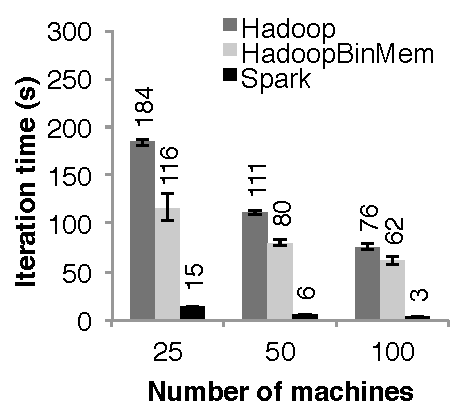
\includegraphics[scale=0.52]{files/lr-later-absol-THIN}%
	}%
	%\hspace{3pt}
	\subfigure[][K-Means]{%
		\label{fig:km-later-absol}%
		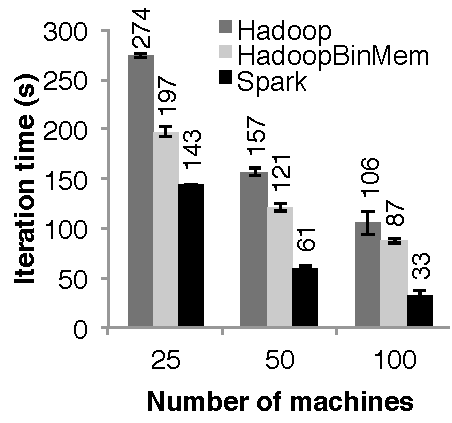
\includegraphics[scale=0.52]{files/km-later-absol-THIN}%
	}%
	%\hspace{8pt}	
	\caption[LR and KM performance]{Runtime comparison}%
	\label{fig:tstm}
\end{figure}

We ran both algorithms for 10 iterations on 100 GB datasets using 25--100 machines. The key difference between the two algorithms is the amount of computation they perform per byte of data. The
iteration time of k-means is dominated by computation, while
logistic regression is less compute-intensive and thus more sensitive
to time spent in deserialization and I/O.

Since typical learning algorithms need tens of iterations to converge,
we report times for the first iteration and subsequent iterations separately.
We find that sharing data via RDDs greatly speeds up future iterations. Note that by the time the user runs the machine learning algorithms in Shark, the working set are likely to be already in memory through the SQL manipulations.

Figure~\ref{fig:tstm} shows how these scaled with cluster size. For logistic regression, Shark was $25.3\times$ and $20.7\times$ faster than Hadoop and \HadoopBM respectively on 100 machines. For the more compute-intensive k-means application, Shark still achieved speedup of $1.9\times$ to $3.2\times$.


%%%%%%%%%%%%%%%%%%%%%%%%%%%%%%%%%%%%%%%%%%%%%%%%%%%%%%%%%%%%%%%%%%%%%%%%%%%%%%%
%%%%%%%%%%%%%%%%%%%%%%%%%%%%%%%%%%%%%%%%%%%%%%%%%%%%%%%%%%%%%%%%%%%%%%%%%%%%%%%
%%%%%%%%%%%%%%%%%%%%%%%%%%%%%%%%%%%%%%%%%%%%%%%%%%%%%%%%%%%%%%%%%%%%%%%%%%%%%%%
\section{Demonstration Details}
\subsection{Demo Setup}
We will present an end-to-end implementation of Shark and demonstrate the benefits it provides. The demonstration exhibits three main components:

\textbf{Data Set}: We will have a HDFS cluster on Amazon EC2 hosting one terabyte (uncompressed) of tweets. It contains roughly 400 million tweets, collected using the Twitter streaming API prior to the conference. These tweets are stored using a nested JSON format.

\textbf{Shark and Hive Clusters}: During the demo, we will have a 100-node Shark cluster and an equal-sized Apache Hive cluster running on EC2 for side-by-side comparison.

\textbf{Web Console}: Since it is hard to capture the internals of query processing given only the query and the output, we have implemented a web console that illustrates the query plan, the caching of RDDs for multi-query optimization, and status of each node. In addition, to demonstrate Shark's fault-tolerance feature, we will arbitrarily submit kill signals to Spark nodes from the web console.

\subsection{Story Line}

Imagine a situation where a data journalist is exploring new topics to write about and at her disposal is a large collection of tweets.

She first generates a histogram of the number of tweets and realizes there is a spike in early October, 2011. Since Twitter activities usually correlate with events, she would like to gain insights about such events by understanding the causes for the spike. To do so, she drills down to focus on the particular two weeks, and clusters tweets by their hash tags. She then realizes there are three large clusters, implying three concurrent events from which the tweets come: the decease of Steve Jobs, the decease of Dennis Ritchie, and the Occupy Wall Street movement.

Suppose she then decides to write a piece about the movement and wants to investigate the public's sentiment towards this movement. Since it is unlikely for the world to have a unanimous view on this particular issue, she would like to compare the distribution of sentiments across different cities: \eg how are people in San Francisco similar to those in New York City? She achieves this by grouping the tweets in this window by geographical location and running the sentiment analysis algorithm. She then uses statistical distribution comparison algorithms to compare the sentiments.

SIGMOD attendees will be able to run queries outlined above as well as perform ad-hoc exploration of the dataset through the command-line interface.

\section{Take-away Message}
This demonstration highlights the benefits of a coarse-grained distributed memory abstraction in allowing deep analysis and interactive querying of massive datasets. Our working prototype provides optimized execution of ad-hoc, exploratory queries that exploit inter-query temporal locality. It additionally provides efficient execution for iterative algorithms that exhibit intra-query temporal locality. We demonstrate Shark's scalability, fault-tolerance and high performance on a realistic analytical workload, while comparing it to Hive. Users will observe the ease of combining deep analysis with SQL, demonstrating how a unified system allows the reuse of intermediate data and significantly improves the performance of analytical queries on massive datasets.

%%%%%%%%%%%%%%%%%%%%%%%%%%%%%%%%%%%%%%%%%%%%%%%%%%%%%%%%%%%%%%%%%%%%%%%%%%%%%%%
%%%%%%%%%%%%%%%%%%%%%%%%%%%%%%%%%%%%%%%%%%%%%%%%%%%%%%%%%%%%%%%%%%%%%%%%%%%%%%%
%%%%%%%%%%%%%%%%%%%%%%%%%%%%%%%%%%%%%%%%%%%%%%%%%%%%%%%%%%%%%%%%%%%%%%%%%%%%%%%

\section{Acknowledgments}
We would like to thank Peter Alvaro, Eric Yi Liu, Tim Kraska, Gene Pang, and Andrew Wang for feedback.

This research is supported in part by gifts from Google, SAP, Amazon Web Services, Cloudera, Ericsson, General Electric, Huawei, IBM, Intel, MarkLogic, Microsoft, NEC Labs, NetApp, Oracle, Splunk, VMware and by DARPA (contract \#FA8650-11-C-7136).

\bibliographystyle{abbrv}
\bibliography{paper}

\balancecolumns
\end{document}
